\documentclass[main]{subfiles}
\begin{document}

\newpage
\chapter*{図表}
\addcontentsline{toc}{chapter}{図表}

% fig and table settings
\renewcommand{\figurename}{Fig. } % 図 -> Fig.
\renewcommand{\tablename}{Table } % 図 -> Fig.

% remove chapter number from (fig. and table) number.
\makeatletter
\@removefromreset{figure}{chapter}
\@removefromreset{table}{chapter}
\makeatother

\def\thefigure{\arabic{figure}}
\def\thetable{\arabic{table}}


\vspace*{\stretch{1}}
\begin{figure}[H]
  \centering
  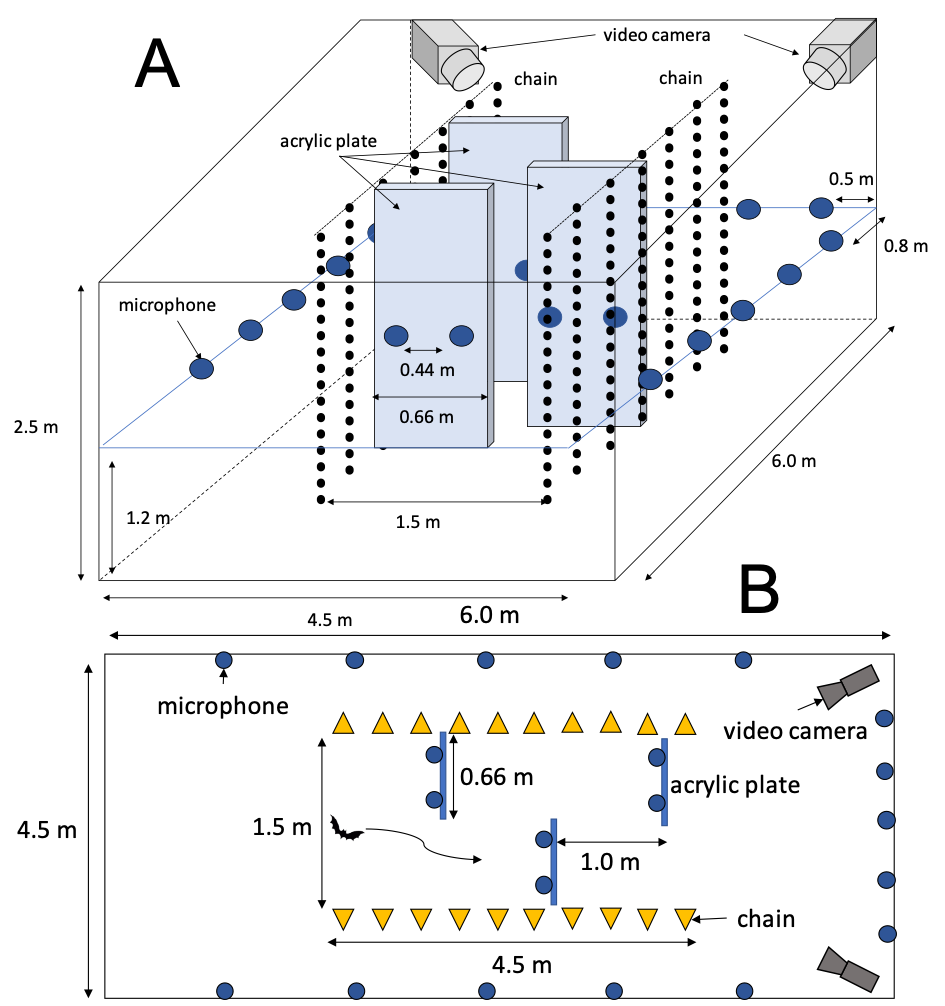
\includegraphics[width=15cm]{figures/top_view_measure.png}
  \caption{
    Top view of measurement system of flight trajectory,
    pulse direction.
  }
  \label{fig:top_view_measure}
\end{figure}
\vspace{\stretch{1}}

\newpage
\vspace*{\stretch{1}}
\begin{figure}[H]
  \centering
  \vfill
  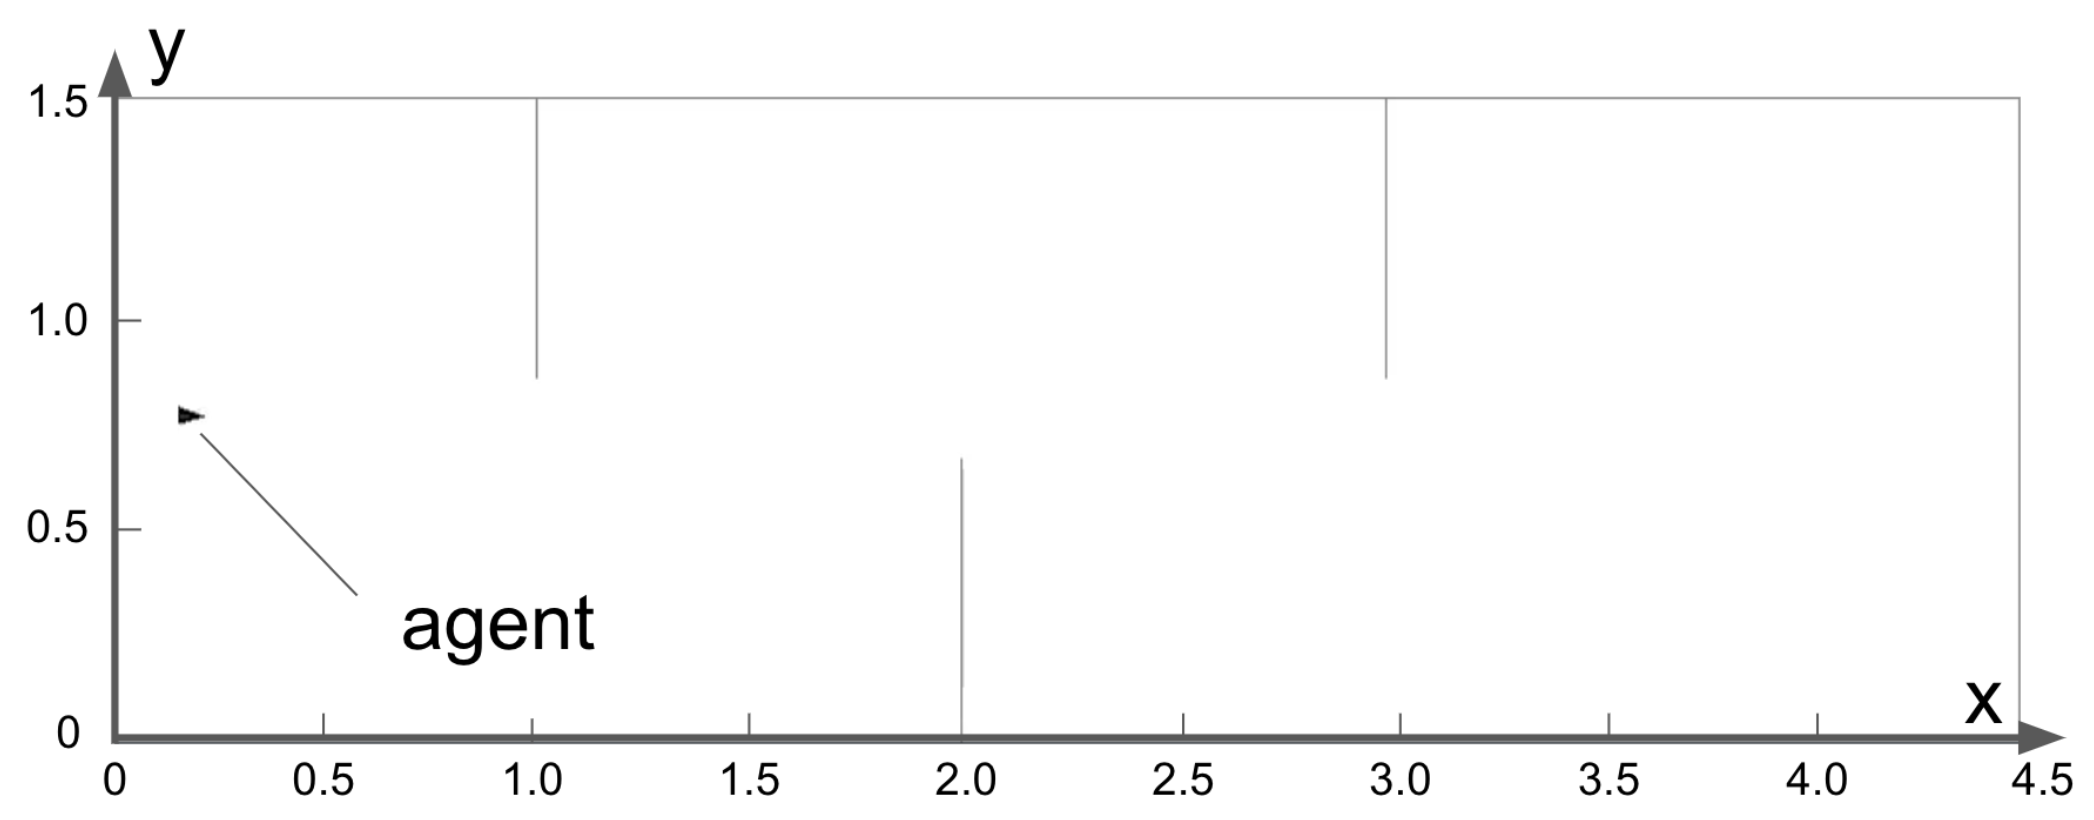
\includegraphics[width=15cm]{figures/simulation_field.png}
  \caption{
    Simulation field.
    Start point for agent is (0.2±0.05, 0.7±0.05).
    The gray lines are obstacles.
  }\label{fig:simulation_field}
\end{figure}
\vspace{\stretch{1}}

\newpage
\vspace*{\stretch{1}}
\begin{table}[H]
  \caption{A, Eの刺激周波数}\label{tab:ae}
  \centering
    \begin{tabular}{c|cl}
      Stimulus Number & Formant frequency\SI{}{[\hertz]} \\
          & F1 & F2 \\ \hline
      1 & 760 & 1080 \\
      2 & 731 & 1656\\
    \end{tabular}
\end{table}
\vspace{\stretch{1}}

\end{document}